%  !TeX  root  =  user_guide.tex

\section{Quick Print Plugin}\label{quickprint}

% when the revision of a section has been finalized, 
% comment out the following line:
% \updatedisclaimer

The \toolbtntwo{quick_print}{Quick Print} Plugin makes it possible to export the current 
map canvas to PDF format quickly and easily, with minimal effort. The only parameters that 
need to be specified are a Map Title, a Map Name, and the Paper Size (See Figure~\ref{fig:quickprint}). 
If you require additional control over the map layout, 
please use the print composer plugin, described in Section~\ref{label_printcomposer}.  

\begin{figure}[ht]
   \begin{center}
   \caption{Quick Print Dialog \nixcaption}\label{fig:quickprint}\smallskip
   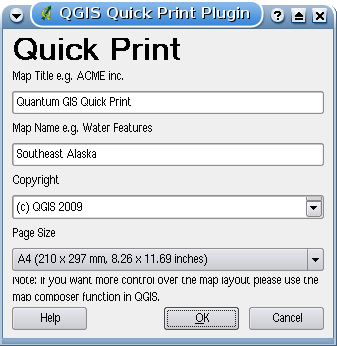
\includegraphics[clip=true, width=6cm]{quick_print_dialog}
\end{center}
\end{figure}

\begin{figure}[ht]
   \begin{center}
   \caption{Quick Print result as DIN A4 PDF using the alaska sample dataset\nixcaption}\label{fig:quickprint_result}\smallskip
   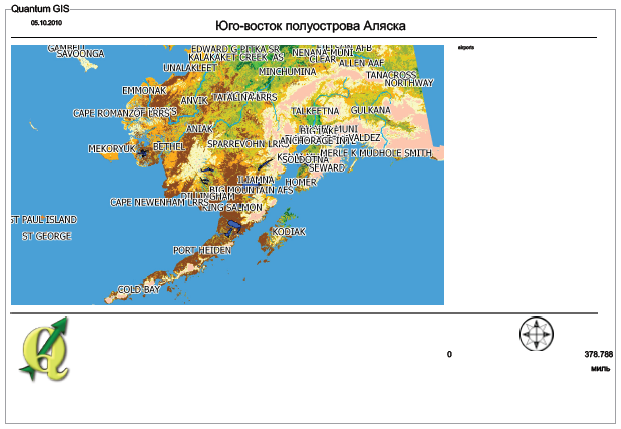
\includegraphics[clip=true, width=9cm]{quick_print_result}
\end{center}
\end{figure}
